\documentclass[12pt,aspectratio=169,english,finnish,pdflatex%,handout
]{beamer}
\definecolor{MyGreen}{RGB}{50, 120, 50}
\usecolortheme[named=MyGreen]{structure}

\usepackage{babel}
\usepackage[utf8]{inputenc}
\usepackage[T1]{fontenc}
\usepackage{amsmath,amssymb} 
\usepackage{animate}
\usepackage{multimedia}

\usepackage{listings}
\usepackage{xcolor}
 
\definecolor{codegreen}{rgb}{0,0.6,0}
\definecolor{codegray}{rgb}{0.5,0.5,0.5}
\definecolor{codepurple}{rgb}{0.58,0,0.82}
\definecolor{backcolour}{rgb}{0.95,0.95,0.92}
 
\lstdefinestyle{mystyle}{
    backgroundcolor=\color{backcolour},   
    commentstyle=\color{codegreen},
    keywordstyle=\color{magenta},
    numberstyle=\tiny\color{codegray},
    stringstyle=\color{codepurple},
    basicstyle=\footnotesize,
    breakatwhitespace=false,         
    breaklines=true,                 
    captionpos=b,                    
    keepspaces=true,                 
    numbers=left,                    
    numbersep=5pt,                  
    showspaces=false,                
    showstringspaces=false,
    showtabs=false,                  
    tabsize=2
}
\lstset{style=mystyle}

\usepackage{natbib}
\bibpunct[: ]{(}{)}{,}{}{}{;}

\usepackage{tikz}

\usepackage{tipa}

\usepackage{hyperref}

\setbeamertemplate{navigation symbols}{}

\graphicspath{{figures/}}

\setlength{\leftmargini}{0pt}
\setlength{\leftmarginii}{1em}

%% Write out the names of graphics files being included 
\newwrite\graphics
\immediate\openout\graphics=\jobname.graphics%
\let\oincludegraphics\includegraphics% store original \includegraphics
\renewcommand{\includegraphics}[2][]{% prepend to it (could also use xpatch, etc.)
  \immediate\write\graphics{#2}
  \oincludegraphics[#1]{#2}}

\newcommand\Wider[2][3em]{%
\makebox[\linewidth][c]{%
  \begin{minipage}{\dimexpr\textwidth+#1\relax}
  \raggedright#2
  \end{minipage}%
  }%
}

\newcommand{\kommentti}[1]{
  {\bf[#1]}
}


\title{Ultraluento
  \\~\\
  Ultraäänen käyttö puheentutkimuksessa
}
\author{Pertti Palo} 
\date{14.4.2026} 


\begin{document}

\frame{\titlepage
  \centering
} 

\frame{\frametitle{Land acknowledgement eli maantunnustus}

I wish to respectfully acknowledge and honor the Myaamiaki (Miami), Lenape
(Delaware), Bodéwadmik (Potawatomi), and šaawanwaki (Shawnee) people, on whose
ancestral homelands I have worked on this presentation.
\vspace{.5cm}

I would also like to respectfully acknowledge that that more recently I have
worked on Treaty 6 territory, which is territory of diverse
Indigenous peoples including the Néhiyaw (Cree), Niitsitapi (Blackfoot), Métis,
Nakoda (Stoney), Dene, Haudenosaunee (Iroquois) and Anishinaabe
(Ojibway/Saulteaux) and many others. 
}

\frame{\frametitle{Kuka tää tyyppi on?}
  \begin{columns}
    \begin{column}{5cm}
      \includegraphics[width=\columnwidth]{uti_eva.png}
    \end{column}
    \begin{column}{5cm}
      \begin{itemize}
      \item Pertti Palo
      \item Minulla on pari tutkintoa Otaniemestä ja viimeisimpänä
        fonetiikan tohtorin paperi.
      \item Puhun sujuvaa foneetikkoa ja insinööriä, ja tiedän paljon
        puheen mittaus- ja analyysimenetelmistä.
      \end{itemize}
    \end{column}
  \end{columns}
} 

% \frame{\frametitle{Johdantoa: Millaisissa (ultraääni) projekteissa olen ollut mukana?}
%   \begin{itemize}
%   % \item Ultraäänellä on tutkittu kielen ja kurkunpään liikkeitä monella eri
%   % tavallla ja ultraääntä on yhdistetty myös muihin mittausmenetelmiin --
%   % esimerkiksi EMA, EEG, EGG ja erityisesti käytännössä aina audio.
%   \item Itse olen keskittynyt puhe-eleiden ajoituksen tutkimiseen aloittaen
%   puheen alun ilmiöistä ja sittemmin tarkastellut koko puhunnosta artikulaation
%   alusta lihasten rentoutumiseen asti.
%   \item Erityisesti olen tehnyt töitä erilaisten metodisten kysymysten parissa.
%   \item Lisäksi olen annotoinut ja murskannut dataa mm.:
%   \begin{itemize}
%     \item Kitahalkion korjaamisen jälkeistä puheterapiadataa,
%     \item Levantin arabiankielen faryngaaliäänteiden vertailudataa, ja
%     \item Eri kielten koartikulaation vertailudataa.
%   \end{itemize}
%   \end{itemize}
% }

\frame{\frametitle{Mitä tuleman pitää}
  \begin{itemize}
  \item Yleistä
  \item Miltä kuva näyttää?
  \item {Kokeillaan käytännössä}
  \item {\usebeamercolor[gray]{} Tauko näillä main}
  \item Tallennussession vaiheet
  \item {Video ultraäänen käytöstä puheterapiassa}
  % \item {\usebeamercolor[gray]{} Ultraäänikuvauksen toimintaperiaate ja ominaisuudet} 
    % \begin{itemize}
  \item {Rajoitteita: Menetelmä ja ihmiset}
    % \end{itemize}
  \item {\bf Kysellään}
  \end{itemize}
}

\frame{\frametitle{Yleistä I}
  \begin{itemize}
  \item Kasvavassa suosiossa puheentutkimuksen parissa.
  \item Puheterapiassa hyödyllinen paitsi välittömän palautteen annossa (osuiko
    liike oikeaan paikkaan) myös tuomassa terapeutille lisätietoa erityisesti
    piilovirheistä.
  \end{itemize}
  
  \centering
  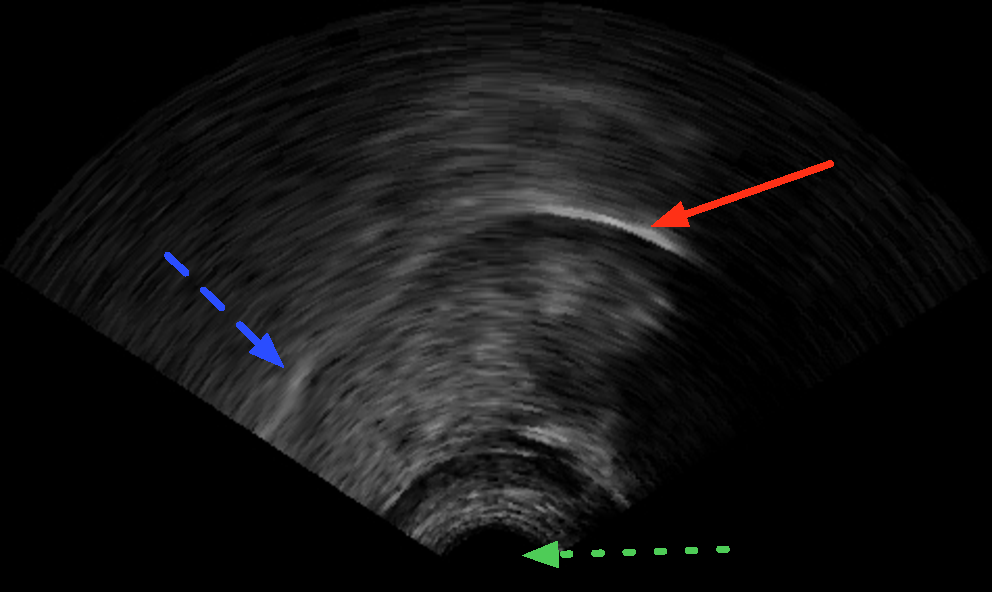
\includegraphics[width=.7\textwidth]{P2_lemon_1st_frame_annotated.pdf}
}


\frame{\frametitle{Yleistä II}
  \vspace*{-2cm}
  \hspace*{6cm}
  
\includegraphics[width=4cm]{batman}
  \vspace{.5cm}
  \begin{itemize}
  \item Lääketieteellisessä ultraäänikuvantamisessa antureilla ja
    niiden erilaisilla ominaisuuksilla on tärkeä rooli.
  \item Ne ovat lähetin-vastaanottimia -- kaikuluotaimia, jotka sekä tuottavat
    että havaitsevat ultraääntä.
  \end{itemize}
  \centering
  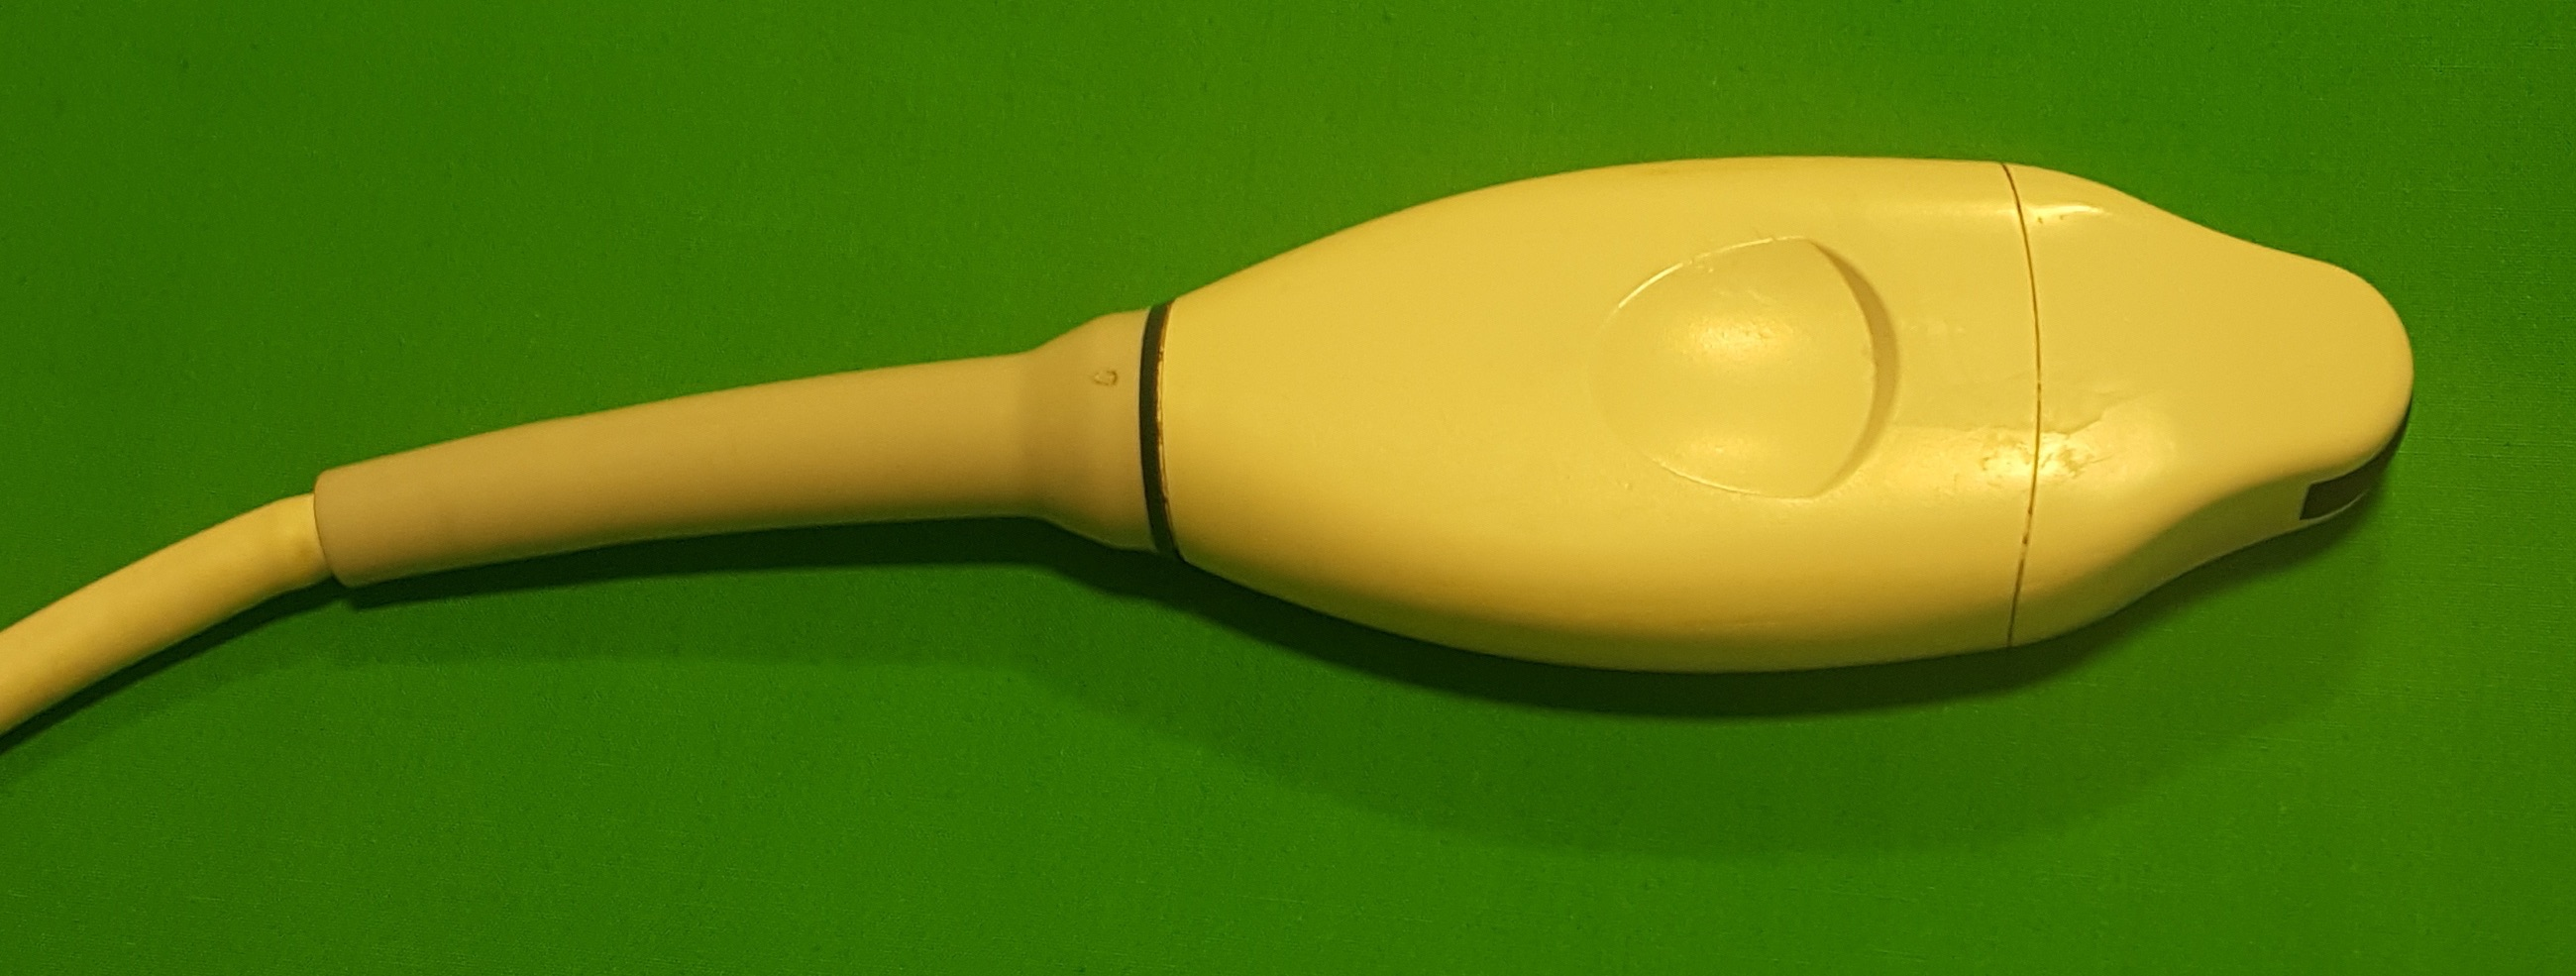
\includegraphics[height=.4\textheight]{probe.jpg}
}

\frame{\frametitle{Miltä kuva näyttää?}
  \centering
  \vfill
  Tavallinen -- kohtuu selkeä -- ultraäänikuva kielestä
  \vfill
  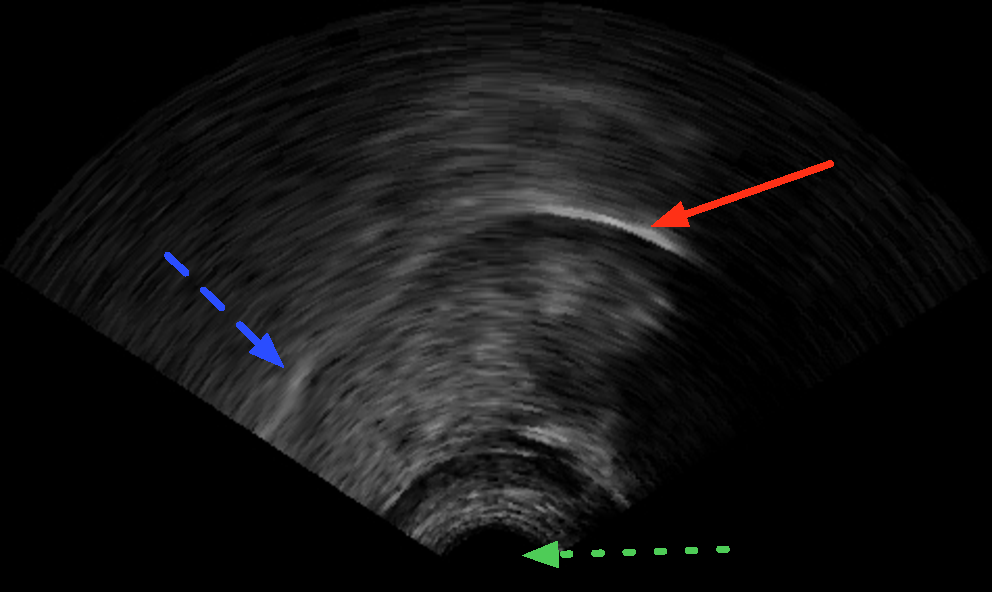
\includegraphics[width=.85\textwidth]{P2_lemon_1st_frame_annotated.pdf}
}

\frame{
  \centering
  {
    \vfill
    \bf \Large 
    \usebeamercolor[fg]{title}
    Puheartikulaation mittaaminen ultraäänellä - kokeillaan
    \vfill
  }
}

\frame{
  \centering
  {
    \vfill
    \bf \Large 
    \usebeamercolor[fg]{title}
    Lyhyt tauko (5 min)
    \vfill
  }
}

\frame{\frametitle{Tallennussession vaiheet}
  \begin{itemize}
  \item Puhdista kaikki.
    \begin{itemize}
    \item Laite on lääketieteellinen koje ja ihmiset ovat likaisia (ja
      korona tappaa).
    \item Aloita pesemällä ja desinfioimalla omat kädet.
    \end{itemize}
  \item Kerro osallistujalle/asiakkaalle kuinka tutkimus etenee, hoida paperihommat, näytä heille kuinka kaikki toimii.
  \item Sovita kypärä osallistujalle päähän, jos kypärä on käytössä.
  \item Tallenna data.
  \item Kerro osallistujalle, että hänestä on ollut paljon apua ja
    auta häneltä kypärä päästä.
  \item Muista antaa käsipyyhkeitä sinisen töhnän poistamiseen
    leuasta.
  \item Puhdista kaikki.
  \end{itemize}
}

\frame{\frametitle{Video ultraäänen käytöstä puheterapiassa}
  \begin{itemize}
    \item Amerikan englannnin puhujille 'normaalius' on sosiaalisesti hyvin
    tärkeää.
    \item Siellä(kin) /r/ on vaikea äänne ja siksi sen kuntouttamiseen nähdään
    paljon vaivaa.
    \item Video on julkaisusta: \linebreak Preston, J. L., McAllister Byun, T., Boyce, S.
    E., Hamilton, S., Tiede, M., Phillips, E., Rivera-Campos, A., \& Whalen, D.
    H. (2017). Ultrasound Images of the Tongue: A Tutorial for Assessment and
    Remediation of Speech Sound Errors. Journal of visualized experiments :
    JoVE, (119), 55123. https://doi.org/10.3791/55123
  \end{itemize}
}

\frame{\frametitle{Etuja I}
  \begin{itemize}
  \item Ultraäänikuvantaminen on hyvin turvallista kun laitetta
    käytetään matalalla tehotasolla.
  \item Ei vaadi ihmeempiä osallistujilta kunhan tallennussessiot
    eivät ole pitkiä.
  \item Helppokäyttöinen -- alkuun tosin laitteiston asentaminen ja
    opetteleminen vaativat työtä.
  \item Laitteisto mahtuu lentokäsimatkatavaraan, mitä on käytetty hyväksi
    kenttätutkimuksessa.
  \item Suhteellisen halpa hankintahinta ja hyvin halvat
    käyttökustannukset.
  \end{itemize}
}

\frame{\frametitle{Etuja II}
  \begin{itemize}
  \item Hyvä aikaresoluutio: Puhekäytössä tavanomaiset laitteet
    tuottavat kuvia 20-120 Hz taajuudella (ja erityisen hyvät
    laitteet jopa 400 Hz taajudella).
  \item Paikkaresoluutiokin on hyvä, mutta monimutkaisempi suure,
    koska resoluutio ei ole vakio kuvan sisällä.
  \end{itemize}
  
  \centering
  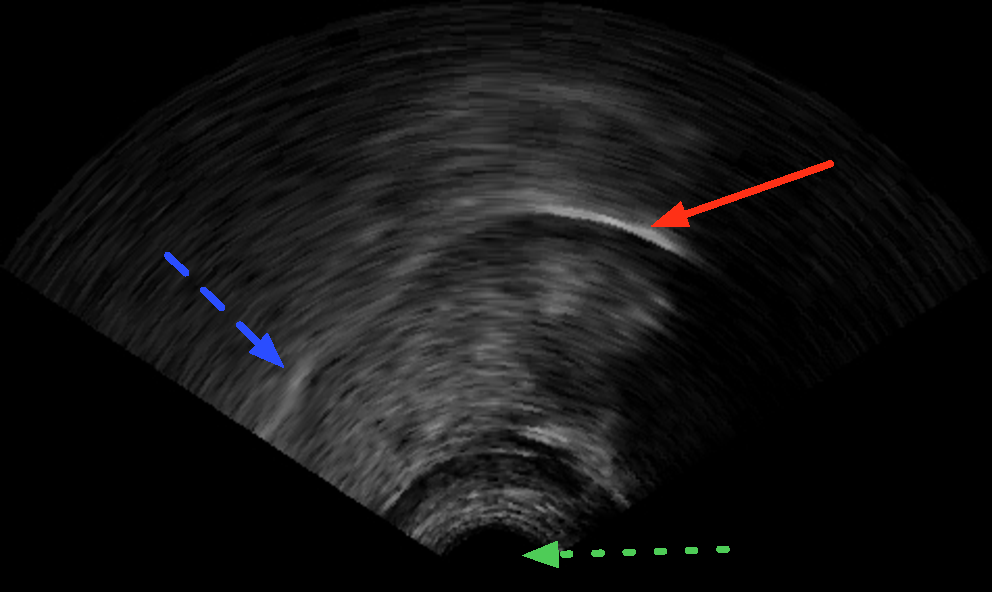
\includegraphics[width=.7\textwidth]{P2_lemon_1st_frame_annotated.pdf}
}

\frame{\frametitle{Rajoituksia I: Kuvanlaatu}
    \begin{itemize}
    \item Aikaresoluutio on kääntäen verrannollinen paikkaresoluutioon.
    \item Resoluutio ja kuvanlaatu riippuvat käytetystä ultraäänen
      taajuudesta: Matalat taajuudet läpäisevät kudokset hyvin, mutta
      tuottavat huonomman paikkaresoluution; korkeat taajuudet
      tuottavat paremman resoluution, mutta eivät läpäise kudoksia
      kovin syvälle.
    \item Erityisesti tottumattomille silmille kuvat ovat suttuisia.
    \item Suttuisuus johtuu suurelta osin kertautuvista kaiuista, kun
      ultraääniaalto heijastelee kudoksen sisällä eri rajapinnoista.
    \end{itemize}
}

\frame{\frametitle{Rajoituksia II: Mitä ylipäätään voidaan kuvata}
  \begin{itemize}
  \item Kaikkia anatomisia rakenteita ei voi kuvantaa ultraäänellä.
  \item Yleensä mistään, mikä on ilmaraon tai luun takana ei saada kuvaa.
  \item Monimutkaiset rakenteet kudosten sisällä voivat tehdä kuvien
    tulkitsemisesta hyvin vaikeaa.
  \end{itemize}
  
  \centering
  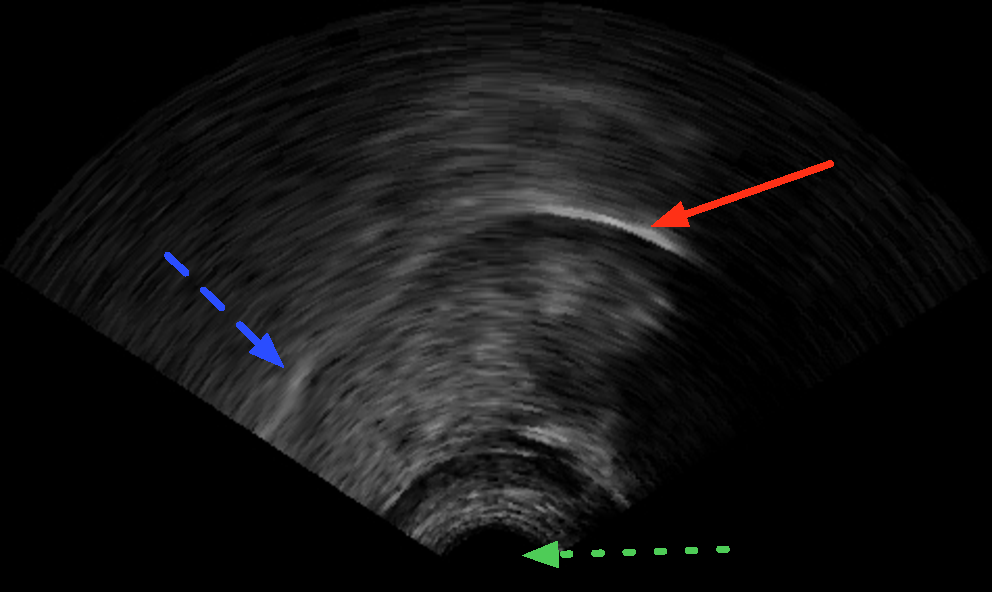
\includegraphics[width=.7\textwidth]{P2_lemon_1st_frame_annotated.pdf}
}

\frame{\frametitle{Rajoituksia III: Menetelmä}
  \vfill
  Anturin vakauttamiseen käytetään erilaisia menetelmiä. Ehkä yleisin on kypärä.
  \vfill
  \begin{columns}
    \begin{column}{.4\textwidth}
      Vanha kypärä -- painaa paljon
      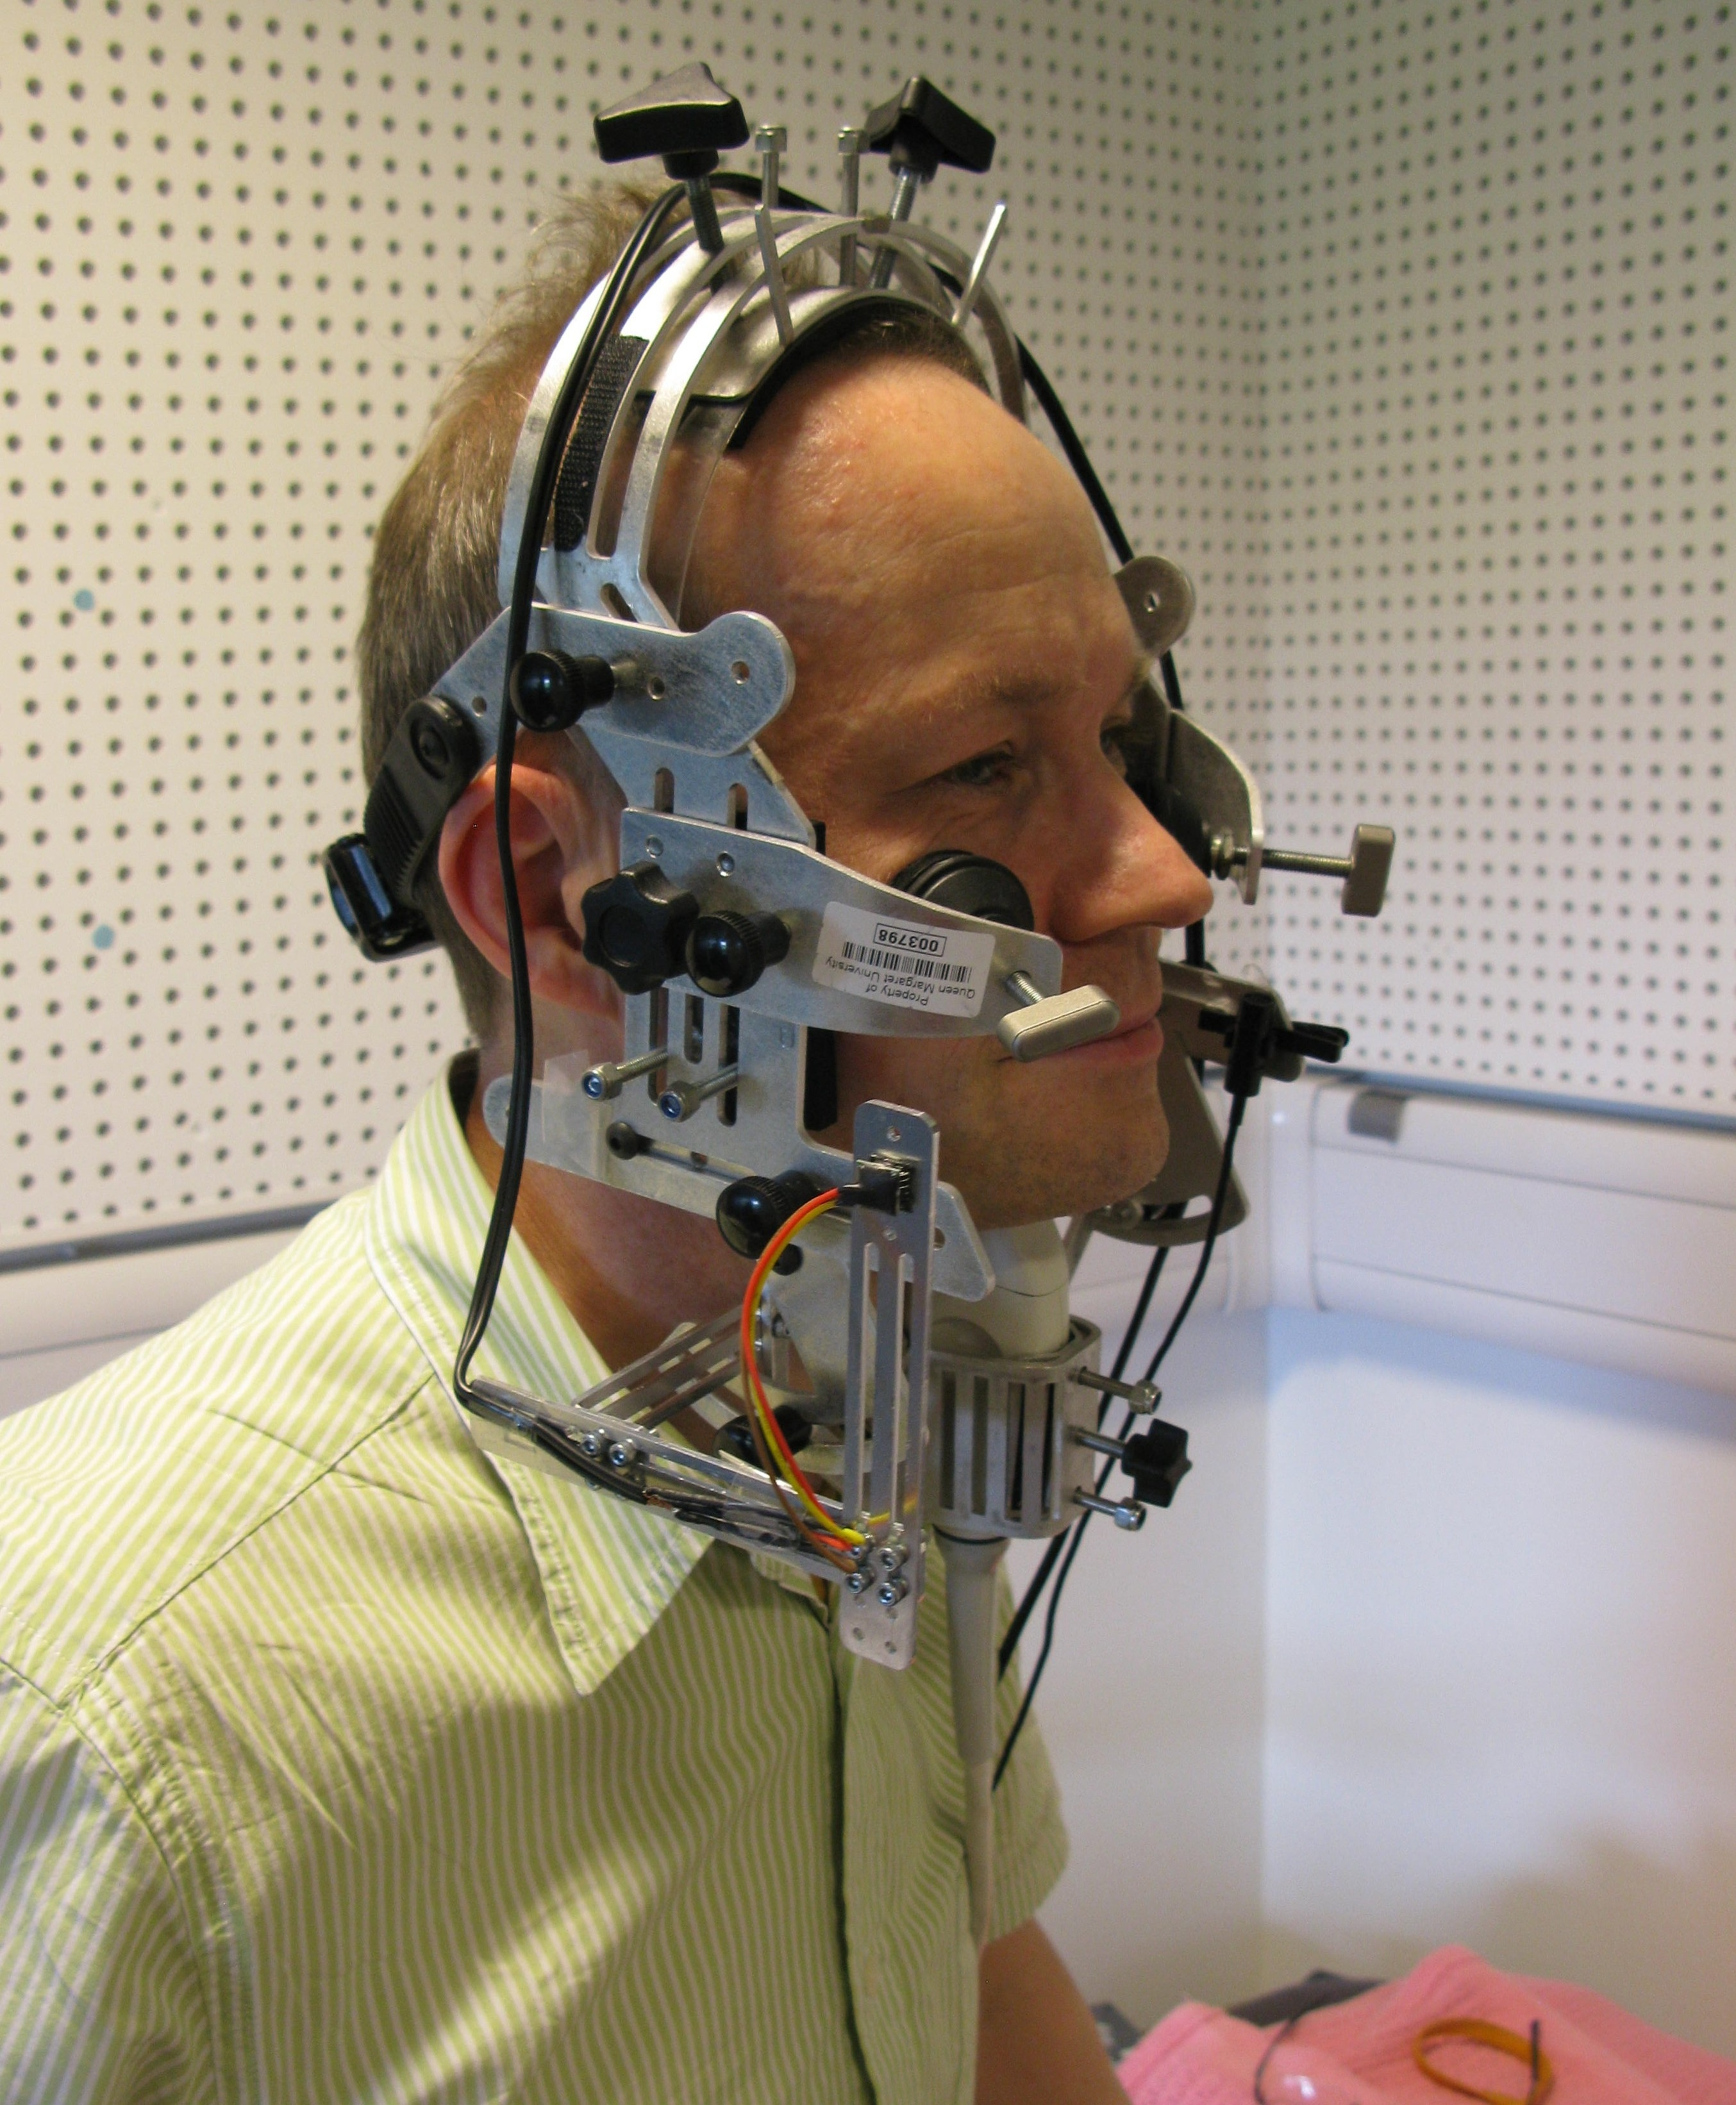
\includegraphics[width=\columnwidth]{UTI_headset.jpg}
    \end{column}
    \begin{column}{.4\textwidth}
      Uusi kypärä -- paljon kevyempi
      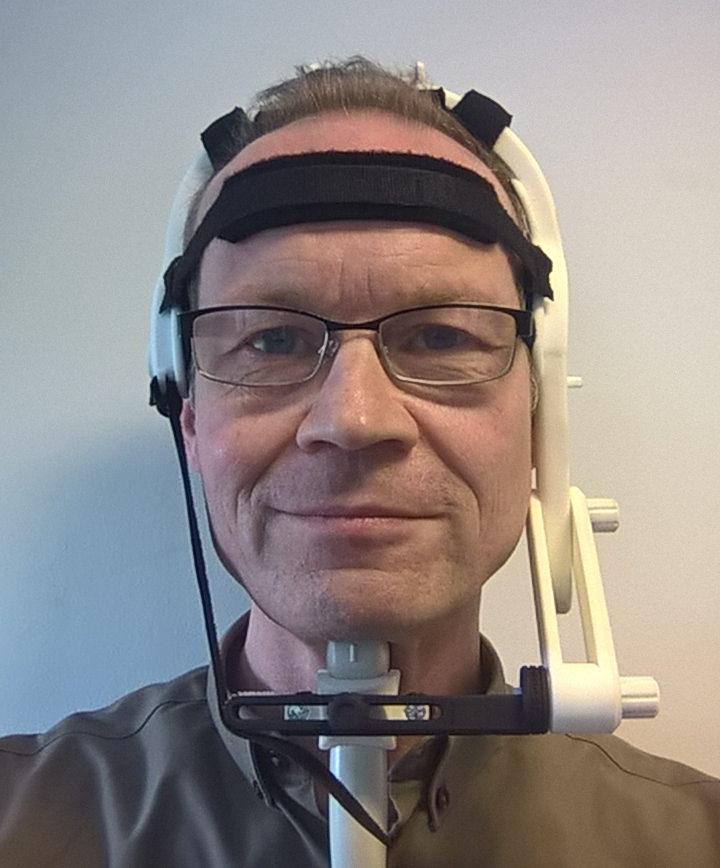
\includegraphics[width=\columnwidth]{UTI_headset_II.png}
    \end{column}
  \end{columns}  
}

\frame{\frametitle{Rajoituksia IV:  Osallistujien valinta}
  \begin{itemize}
  \item Pienet lapset eivät voi käyttää kypärää ja lapsia ylipäänsä
    on vaikea motivoida olemaan riittävän paikoillaan.
  \item Anturia voidaan pitää kädessä, mutta käsin vakautettu data
    on vaikeampaa analysoida.
  \item Suuripäiset, erityisesti suurikieliset ihmiset kuvantuvat
    huonosti.
  \item Suuri määrä rasvakudosta leuan alla tekee kuvantamisesta
    haastavaa.
  \item Ikä lisää kiinnikkeiden määrää mm. kielen
    sisällä. Kiinnikkeet aiheuttavat suttua kuvassa.
  \end{itemize}
}


\frame{
  \centering
  {
    \vfill
    \bf \Large 
    \usebeamercolor[fg]{title}
    Kyselkää
    \vfill
  }
}


\frame{\frametitle{Kiitokset}

  \begin{itemize}
  \item Steve Cowen: AAA:n käyttöapu ja kuva minusta.
  \item Felix Schaeffler: lepakkokuva.
  \item Alan Wrench: AAA:n käyttöapu ja laitteistokuvat.
  \item Megan Diekhoff: Kliinisen tutkimuksen vinkit.
  \end{itemize}
}

\end{document}

\frame{
  \centering
  {
    \bf \Large 
    \usebeamercolor[fg]{title}
    Something else i.e. section title
    
    \vfill
%    \includegraphics[height=1.5cm]{figures/aalto_logo} 
  }
}


